\documentclass[12pt,english]{article}
\usepackage[a4paper,bindingoffset=0.2in,%
            left=1in,right=1in,top=1in,bottom=1in,%
            footskip=.25in]{geometry}
\usepackage{blindtext}
\usepackage{titling}
\usepackage{amssymb}
\usepackage{amsmath}
\usepackage{listings}
\usepackage{lettrine} 
\usepackage{tikz}  
\usepackage{color} 
 \usetikzlibrary{shapes, arrows, calc, arrows.meta, fit, positioning} % these are the parameters passed to the library to create the node graphs  
\tikzset{  
    -Latex,auto,node distance =0.6 cm and 1.3 cm, thick,% node distance is the distance between one node to other, where 1.5cm is the length of the edge between the nodes  
    state/.style ={ellipse, draw, minimum width = 0.9 cm}, % the minimum width is the width of the ellipse, which is the size of the shape of vertex in the node graph  
    point/.style = {circle, draw, inner sep=0.18cm, fill, node contents={}},  
    bidirected/.style={Latex-Latex,dashed}, % it is the edge having two directions  
    el/.style = {inner sep=2.5pt, align=right, sloped}  
}  
\setlength{\parskip}{12pt}
\title{Home Work 1}
\date{\today}
\author{Jose Carlos Munoz}
%================================
\begin{document}
\newgeometry{left=0.8in,right=0.8in,top=1in,bottom=1in}
\begin{center}
    \Large
    \textbf{Homework 1}\\
    \small
    \today\\
    \large
    Jose Carlos Munoz
\end{center}\par
%In the middle if you want to change the margins use
1)3.9.a] state format [mL cL P mR cR]\\
mL: number of missionaries on the left bank\\
cL: number of cannibals on the left bank\\
P: Location of the boat (L or R)\\
mR: number of missionaries on the right bank\\
cR: number of cannibals on the right bank\\
\begin{center}
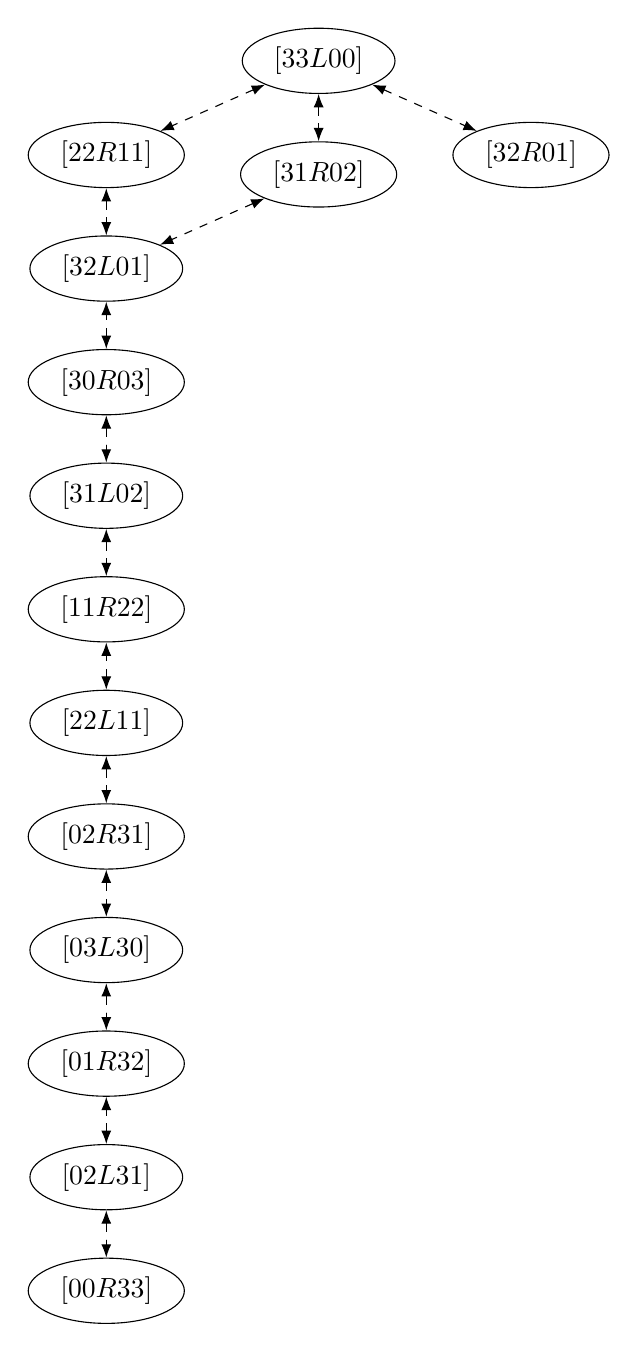
\begin{tikzpicture}  
    % a is the name of the node and A is the text inside the node/vertex  
    \node[state] (a) at (0,0) {$[33L00]$}; % here, state signifies that the shape of the node will be the shape declared in the above state/.style command.  
  
    % you can mention any location such as right, left, above, below, etc.  
     
    \node[state] (b) [below left =of a] {$[22R11]$};  
    \node[state] (c) [below =of a] {$[31R02]$};  
	\node[state](d)[below right = of a]{$[32R01]$};
	\node[state](e)[below =of b]{$[32L01]$};
	\node[state](f)[below =of e]{$[30R03]$};
	\node[state](g)[below =of f]{$[31L02]$};
	\node[state](h)[below =of g]{$[11R22]$};
	\node[state](i)[below =of h]{$[22L11]$};
	\node[state](j)[below =of i]{$[02R31]$};
	\node[state](k)[below =of j]{$[03L30]$};
	\node[state](l)[below =of k]{$[01R32]$};
	\node[state](m)[below =of l]{$[02L31]$};
	\node[state](n)[below =of m]{$[00R33]$};	  
    % Bidirected edge  
     \path[bidirected] (a) edge[bend right=0] (b);  
     \path[bidirected] (a) edge[bend right=0] (c);  
     \path[bidirected] (a) edge[bend left=0] (d);  
     
     \path[bidirected] (b) edge[bend left=0] (e);  
     \path[bidirected] (c) edge[bend left=0] (e);  
     
     \path[bidirected] (f) edge[bend left=0] (e);  
      \path[bidirected] (f) edge[bend left=0] (g);  
      
     \path[bidirected] (g) edge[bend left=0] (h);  
     \path[bidirected] (i) edge[bend left=0] (h);    
     \path[bidirected] (i) edge[bend left=0] (j);  
     \path[bidirected] (j) edge[bend left=0] (k);
     \path[bidirected] (k) edge[bend left=0] (l); 
     \path[bidirected] (m) edge[bend left=0] (l);  
     \path[bidirected] (m) edge[bend left=0] (n);
\end{tikzpicture}
\end{center}\par
2)3.9.b] the Start state is [33L00] and the goal state [00R33]. Since the state graph loops back, it is better to use a graph tree and record the nodes that we have already visted.\\
frontier(0) [[33L00]]$\rightarrow$ frontier(1) [[22R11] [31R02] [32R01]]$\rightarrow$  frontier(2) [[32L01] [31R02] [32R01]]$\rightarrow$\\ 
frontier(3) [[32L01] [32R01]]$\rightarrow$ frontier(4) [[32L01]]$\rightarrow$  frontier(5) [[30R03]]$\rightarrow$\\ 
frontier(6) [[31L02]]$\rightarrow$ frontier(7) [[11R22]]$\rightarrow$  frontier(8) [[22L11]]$\rightarrow$  frontier(9) [[02R31]]$\rightarrow$\\ 
frontier(10) [[03L30]]$\rightarrow$ frontier(11) [[01R32]]$\rightarrow$  frontier(12) [[02L31]]$\rightarrow$  frontier(13) [[00R33]]\par
3)3.18] If the goal of state was in the deeper nodes of the first options, then iterative depth search will take a longer time to reach it than a Depth first search.\par
3.21.a] Uniform cost search always expands the nodes with the loweset step cost. If the step cost is the same for all the following nodes, then it will act as  Breadth-First search. We can then say that a Breadth-First search is a special case of the unofrm cost search when the step cost g(v) is the same for all nodes.\par
3)3.21.b] A Depth-First serach as the same as a the best first tree search when each breanch it epands is the lowest.\par
3)3.21.c] The A* search has a total cost function of f(v) = g(v) + h(v);where g(v) is the step cost and h(v) is the estimate cost to goal state. The Uniform Cost search expands the nodes with the lowest step cost(g(v)). So an A* search can act like a Uniform Cost search when the  h(v) = 0 for all the nodes.  We can then say that the Uniform Cost search is a special case of the A* search.\par
4) The heuristic function of a the manhattan distace is admissable because it takes into account only when a certain tile is in place the correct place. As it gets close to its correct place, the f(v) $\leq$ C*(v). This heuristic function also shows when v' is the child of v, we can see that the h(v) $\leq$ c(v,v') + h(v'), due to the triangle inequality.\par
5) Lets say that $h_1$ is the hueristic function of how many tiles are out of place and $h_2$ is the heuristics function of total distance away from its correct positon. $h_1$ only takes into account how many tiiles are in place, however it doesn't take into account how far away the tile is away from its goal position. This means that it treats a tile that is only 1 step away that same as one that is n steps away.\par
The $h_2$ takes this distane into account. Therefore, it will choose moves that are closer to the correct location. This will take less steps being much more accurate.
%===============================
\end{document}